\documentclass[11pt]{article}

\usepackage{amssymb}
\usepackage{amsthm}
\usepackage{amsmath}
\usepackage[utf8]{inputenc}
\usepackage{mathabx}
\usepackage{framed}
\usepackage{booktabs}
\usepackage{mathtools}
\usepackage{hyperref}
\hypersetup
	{ 
		colorlinks=true,       % false: boxed links; true: colored links
%		hidelinks,
		linkcolor=blue,          % color of internal links (change box color with linkbordercolor)
		citecolor=green,        % color of links to bibliography
		filecolor=magenta,      % color of file links
		urlcolor=cyan,           % color of external links
		linkbordercolor	= {1 0 0},
		citebordercolor	= {0 1 0},	
		urlbordercolor	= {0 1 1}
	}


\usepackage{fontspec}
%\setmainfont{Clear Sans}
%\newfontfamily{\clearsans}{Clear Sans}

\newcommand{\definition}{\\ \textbf{Definition:} \hspace{1cm} }

\newcommand*{\QEDA}{\hfill\ensuremath{\blacksquare}}%
\newcommand*{\QEDB}{\hfill\ensuremath{\square}}%


\begin{document}
	\title{Experimental Physik II Kapitel 15}
		\author
		{
			author\\
			{\small 	\texttt{email}}
		}
		\date{\today}
	\maketitle
	\tableofcontents
	\setcounter{section}{14} %Hier fängt die Nummerierung an.
	
	\newpage
	
\section{Stationäre El. Ströme }
	\subsection{}
		\textbf{Definition:} \hspace{1cm} Elektrischer Strom := Bewegung von el. Ladung \\
		\\
		Stromst\"{a}rke $\textbf{I} = \frac{dQ}{dt}$ [I] =[$\frac{Ladung}{Zeit}$] $=\dfrac{C}{s} = A$ \\
		Stationäre Ströme: Keine explizite Zeitabhängigkeit.\\ 
		\\
		\textbf{Definition:} \hspace{1cm} El. Stromdichte \textbf{j} \\
		$j:=\frac{Ladung}{Zeit\cdot Flaeche} $ [$j$] $=\dfrac{A}{m^2}$ \\
		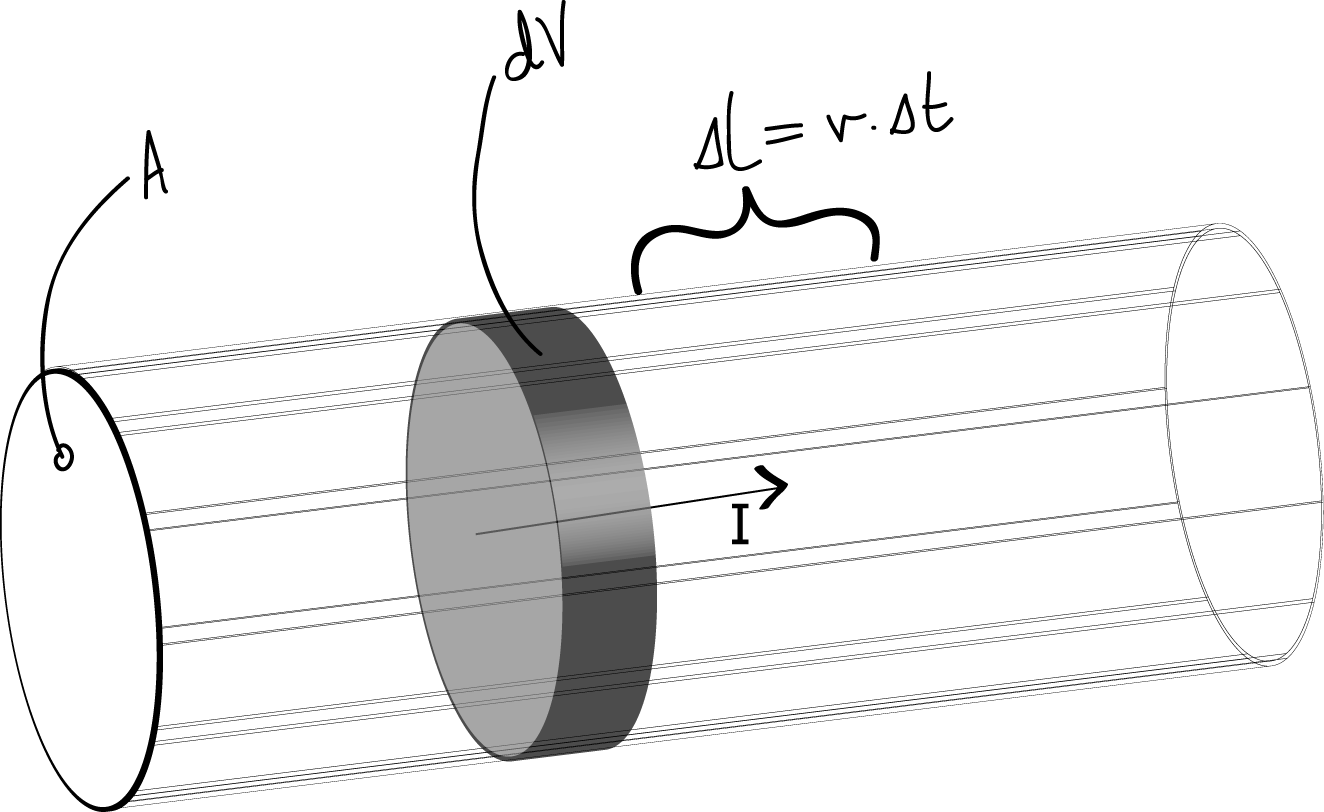
\includegraphics[width=0.6\linewidth]{skizzen/15/VL06/15_1}
		\\
		
		\noindent$N=n\cdot \Delta V $ Ladungsträger \marginpar{($n$ ist die Ladungsträgerdichte)} mit der Ladung q treten im Zeitintervall $\Delta t$ durch $\diameter$-Fläche A. \\
		\\
		Annahme: Alle Ladungen haben die gleiche Geschwindigkeit \emph{v}, dann ist die transportierte Ladung:
		$$\Delta Q=N\cdot q = n\cdot \Delta V \cdot q = n\cdot q \cdot A \cdot \Delta l = n \cdot q\cdot A\cdot v \cdot \Delta t$$
		$$j=\frac{\Delta Q}{\Delta t \cdot A}=n\cdot q \cdot v =  \rho \cdot v $$ \begin{flushright}
			$\rho$ := Ladungsdichte [$C/m^3$]
		\end{flushright}
		{\large \textbf{Allgemein: } \boxed{\vec{j} = \rho \cdot \vec{v} }} \\
		\newpage
		Stromdichte $\longrightarrow$  Stromstärke: $I = {\displaystyle \int\limits_A} \vec J \cdot \mathrm d\vec A$ \\
		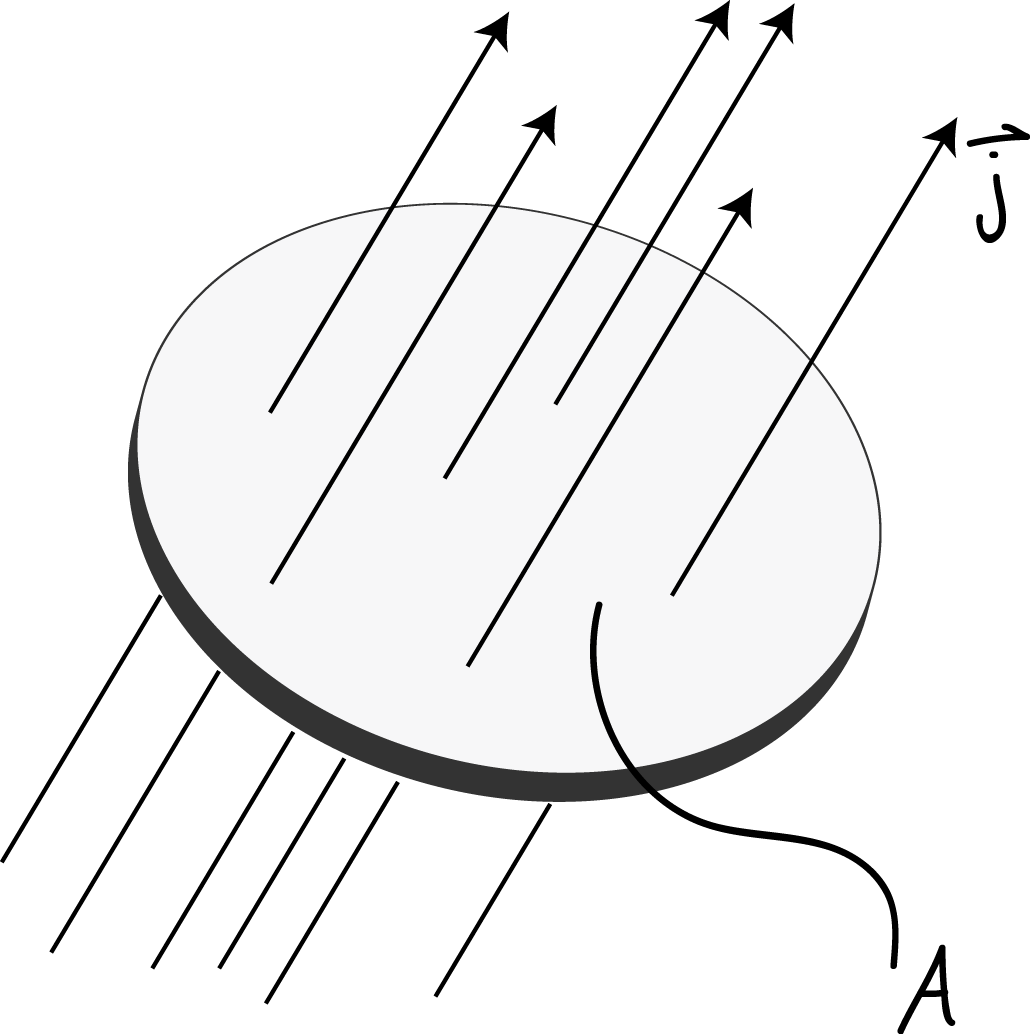
\includegraphics[width=0.3\linewidth]{skizzen/15/VL06/15_2} \\
		\paragraph{\underline{Kontinuitätsgleichung:}}
		Geschlossene Fläche \emph{A} umschließt Volumen \emph{V}.
		$$\underline{I = {\displaystyle\oint\limits_A} \vec{j} d\vec{A} = -\frac{dQ}{dt} = -\frac{d}{dt} \overbrace{{\displaystyle\int\limits_V} \rho \hspace{1mm} dV}^{=Q} }$$
		Differenz zwischen ein. und ausgeströmter Ladung entspricht der negativen Änder der Gesamtladung im Volumen! \\
		($\Rightarrow$ Ladungserhaltung) \\
		\rule{\textwidth}{0.2mm}
		\subsection{\underline{Das Ohmsche Gesetz}}
		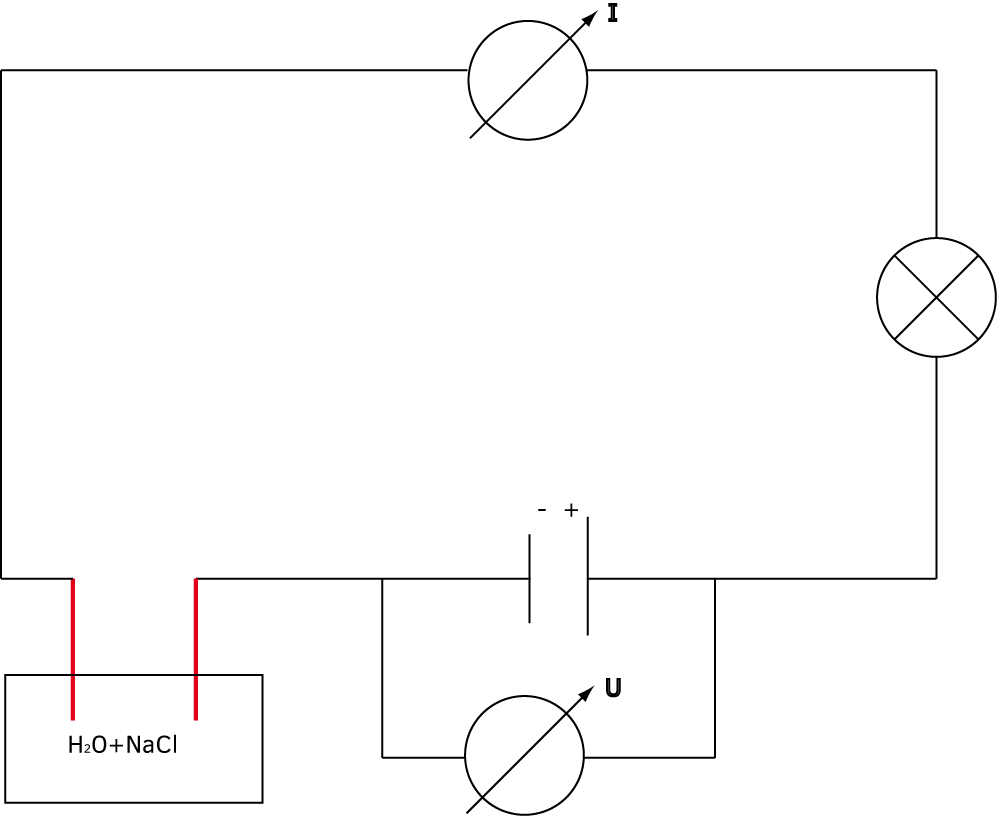
\includegraphics[width=0.7\linewidth]{skizzen/15/VL06/15_3} \\
		$\Rightarrow$ freie Ladungsträger (Ionen) notwendig, damit Strom fließt. \\
		$\Rightarrow$ Dissoziation von $NaCl$ in $Na^+$ und $Cl^-$ \\
		Coulombkraft $|\vec{F_c}| = \frac{1}{4\pi\epsilon_0} \cdot \frac{q_1 \cdot q_2}{r^2} \cdot \frac{1}{\epsilon}$ \\
		$\epsilon_{H_2O}\approx 80 \Rightarrow$ Reduktion von $F_c$ in $H_2o$\\
		\begin{center}
			$\Rightarrow$ \underline{Dissoziation möglich!}
		\end{center}
		qualtitatv: $I \sim U$ \\
		Ersetze Elektrolyt durch Metallwiederstand! \\
		$$I\propto U$$
		\\
		\paragraph{Ohmsches Gesetz:} Wird eine Potenzialdifferenz U and das Ende eines el. Leiters appliziert, so fließt ein el. Strom \emph{I}, dessen Stromstärke proportional zu \emph{U} ist. \\
		{\large $$\boxed{ I = \frac{1}{R} \cdot U }$$} \\
		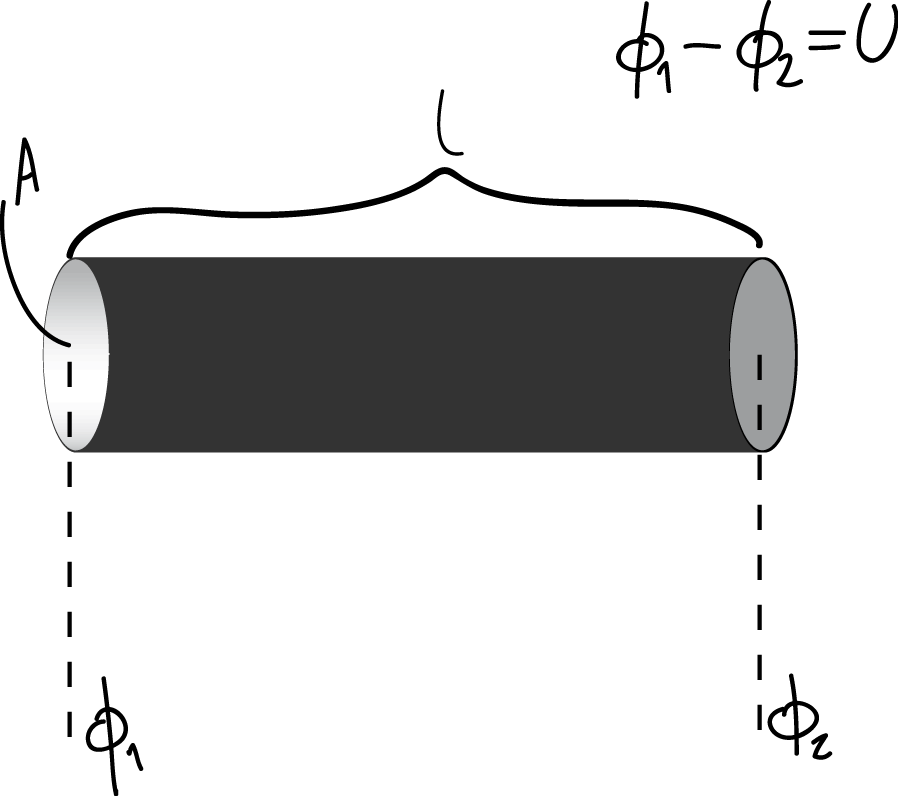
\includegraphics[width=0.8\linewidth]{skizzen/15/VL06/15_4} \\
		Empirischer Befund:
		\begin{align*}
		I &\sim (\phi_2-\phi_1) \\
		I &=\frac{1}{R} (\phi_2-\phi_1) \\
		&= \frac{A}{l} \cdot \frac{1}{\rho} (\phi_2-\phi_1)
		\end{align*}
		
		\noindent \definition $\boxed{R:= \rho \cdot \frac{l}{A}}$ el. Widerstand [\emph{R}] $= \frac{V}{A} = \Omega =$ 1 Ohm \\
		$\rho$: Materialkonstante: spezifischer el. Widerstand [$\rho$] $=\Omega m$ \\
		$\frac{l}{A}$: Geometrieparameter \\
		{\large Ohmsches Gesetz: $\boxed{I=\frac{U}{R}}$} \\
		$\frac{I}{A}=\frac{1}{\rho }\cdot \frac{{\varphi }_{2}-{\varphi }_{1}}{l}$ \\
		$\left|\vec{j}\right|=\frac{1}{\rho }\cdot \left|\vec{E}\right|$ \hspace{2cm} $\frac{1}{\rho} = \sigma := $ el. Leitfähigkeit [$\sigma$] = $Ohm^{-1} m^{-1} = \frac{A}{Vm}$ \\
		$|\vec{j}| = \sigma \cdot |\vec{E}|$ \\
		Empirischer Befund: $\boxed{\vec{j_m} = \sigma_{mn} \vec{E_n} }$ Allegemeines Ohmsches Gesetz\\
		\newpage
		\noindent Mikroskopische betrachtung - Drende Modell \\
		Metall: positiv geladene Atomrümpfe; Elektronen dazwischen beweglich. \\
		
		a.) ohne potenzialdifferenz: thermische ungeorndete bewegung.\\
		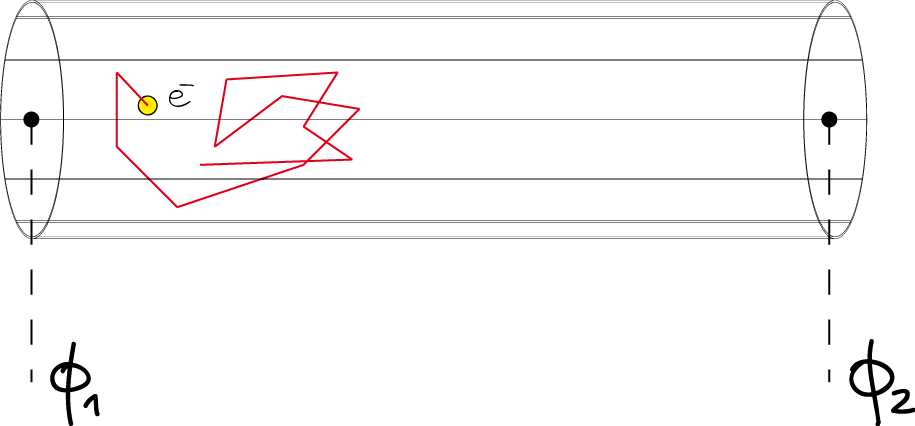
\includegraphics[width=10cm]{skizzen/15/VL06/15_5} \\
		\break
		$ <\vec{v}> = 9 \Rightarrow  $ Im Mittel kein Transport\\
		\begin{align*}
		\text{obwohl: } \sqrt{<v^2>} = \frac{\sqrt{3 K_BT}}{m_e} &\approx 10^5 \frac{m}{s} \\
		&\text{bei } (T=RT) 
		\end{align*}
		b.) $ \phi_2 - \phi_1 \neq 0 \Rightarrow $ El. Feld im Leiter \\
		Zwischen Stößen Beschleunigt durch el. Feld: \\
		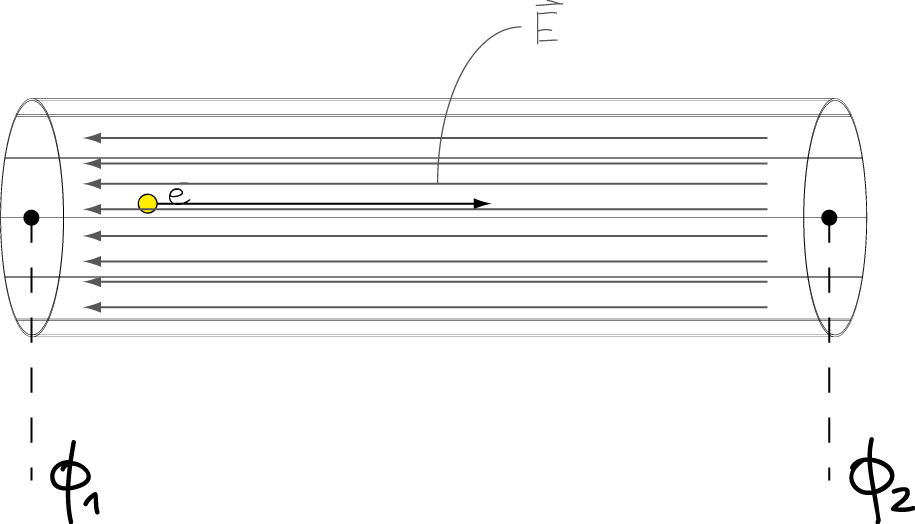
\includegraphics[width=10cm]{skizzen/15/VL06/15_6}\\
		\break
		$\Rightarrow$ \emph{"Drift"} mit Geschwindigkeit $v_D$, die der thermischen Bewegung überlagert ist. \\
		\begin{flalign*}
		\text{Kraft auf Elektron: } \vec{F} &= q_{el} \cdot \vec{E}&&\\
		\Rightarrow \vec{a} &= \frac{q_{el}}{m} \cdot \vec{E}&& \\
		\Rightarrow \vec{v_D} &= \frac{q_{el}}{m} \cdot \vec{E} \cdot \Delta t&& \\
		\end{flalign*} 
		\begin{flalign*}
		\text{ Betrachte Ohmsches Gesetz. } &&\\
		\vec{j} = \sigma \cdot \vec{E} ; \vec{j} = q_{el} \cdot n \cdot \vec{v_D}&& \\
		\text{\underline{Beträge:} } j = \frac{q_{el} \cdot n \cdot v_D}{E} \cdot E = \sigma \cdot E&& \\
		\Rightarrow \sigma = \frac{n\cdot q_{el} \cdot v_D}{E} = const.&& \\
		\Rightarrow \frac{|\vec{v_D}|}{|\vec{E}|} = const.&& \\ 
		\end{flalign*}
		$ |\vec{v_D}|=\mu \cdot |\vec{E}| $ \hspace{1cm} $ \mu $: Beweglichkeit (unabh. von $ \vec{E} $)! \\
		$$ \boxed{\sigma = n\cdot q_{el} \cdot \mu  } $$
		\begin{center}
			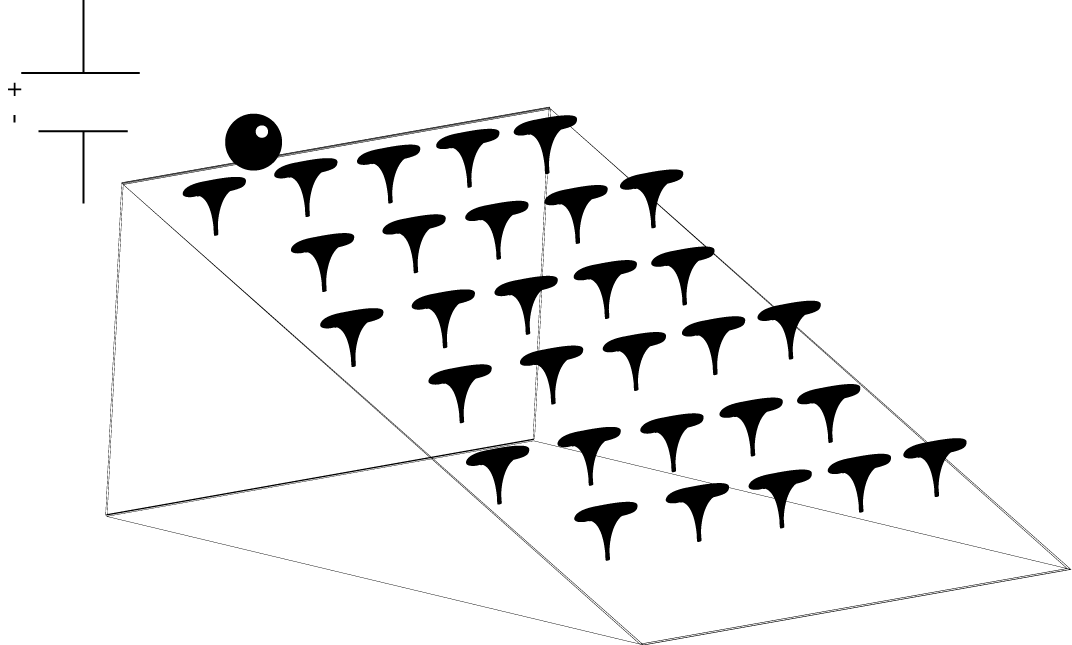
\includegraphics[width=0.5\linewidth]{skizzen/15/VL06/15_7}
		\end{center}
		Damit sich im el. Feld ein Konstates $ v_D $ einstellt, muss es etwas geben\marginpar {$ \Rightarrow $Exp.Phy.I: Stokes-Reibung} wie geschwindigkeitsabhängige Reibung! \\
		$ \Rightarrow $ Makroskopisch: (1-dim) \\
		$$ m\ddot{x}+\frac{m}{\tau}\dot{x} = q_{el}E$$
		$$\boxed{\dot{x} =\frac{q_{el}}{m} \cdot E \cdot \tau \cdot (1-exp(-t/t))}$$
		$ \tau $; Relaxationszeit: Gibt an, nach welcher Zeit \emph{v} auf \emph{v/e} abgenommen hat. \\
		$ \Rightarrow $ \underline{Mikroskopisch:} \\
		$ \tau $: Zeit zwischen zwei Stößen ("Stößzeit") \\
		
		\begin{align*}
		\Rightarrow m \cdot \vec{v_D} = q_{el} \cdot \vec{E} \cdot \tau \\
		\Rightarrow \vec{j} = n\cdot q_{el} \cdot \vec{v_D} = \underbracket[0.5pt][7pt]{\frac{n \cdot q_{el}^2 \cdot \tau}{m}}_{\boxed{\underset{\text{Drude-Leitfähigkeit}}{\sigma = \frac{n \cdot q_{el}^2 \cdot \tau}{m}}}} \cdot \vec{E}\\
		\Rightarrow \boxed{\mu = \frac{q_{el}\cdot \tau}{m}} \hspace{1cm} \text{[$\mu$]} = \frac{m^2}{Vs}
		\end{align*}
		$ \Rightarrow $ Voraussetzung für Gültigkeit des Ohmschen Gesetz:
		\begin{enumerate}
			\item Transport durch Stöße dominiert
			\item \emph{n} unabhängig von $ \vec{E} $
			\item $ \tau $ unabhängig von $ \vec{E} $
		\end{enumerate}
		$ \tau $ klein $\Rightarrow$ $ v_D $ klein (und beobachtbar!) 
		\newpage
				

\end{document}
